Lors de l'installation du plugin, deux menus s'ajoutent sur la partie \textit{back-office}. Le premier se trouve dans le menu \textbf{Édition} et le deuxième dans le menu \textbf{Configuration}. 

\subsection{Menu configuration} \label{subsection:configuration}

Dans le menu configuration se trouvent trois sous-menus :
\begin{itemize}
    \item Diverses options
    \item Gestion des rôles
    \item Gestion des notifications
\end{itemize}
Nous allons revenir sur ces différents menus.

\subsubsection*{Diverses options} \label{subsubsection:diverses-options}
Dans ces sous-menus, il est possible de définir différents paramètres. Ces paramètres sont censés offrir des possibilités d'adaptation du plugin aux besoins du site. Nous allons les expliquer un par un. Pour chaque configuration, le système de configuration SPIP a été utilisé. Les configurations sont donc accessible dans le code via les fonctions \texttt{ecrire\_config} et \texttt{lire\_config}.\\
\newline
Le fichier \texttt{action/exemple\_configuration.php} offre une configuration d'exemple déjà définie. Il est possible de l'utiliser en passant par le bouton du menu nommé "\textit{Utiliser la configuration d'exemple}". Cependant il est toujours préférable de réaliser une configuration adaptée au site.\\
\newline
Pour chaque configuration, la valeur prend soit 0, soit 1. Si la valeur est à 0 (valeur initiale) alors l'option n'est pas activée, sinon, si l'option est sur 1, alors elle est activée.

\newpage
% ///////////////////////////////////


\textbf{Option 1 :} 
\begin{itemize}
    \item Configuration : \texttt{osi\_projets/rubriques/N} avec N l'indice de la rubrique
    \item Explication : Cette option comporte deux groupes de rubrique, le premier groupe représente les rubriques classiques et le deuxième groupe représente toutes les rubriques dans lesquelles il est possible de créer un projet sur le front (sans parler de sous projet, Cf option \ref{option9}. Il n'est pas nécessaires qu'une rubrique soit une rubrique de création pour voir ses sous projets)
\end{itemize}
\vspace{0.5cm}
\begin{figure}[h]
    \centering
    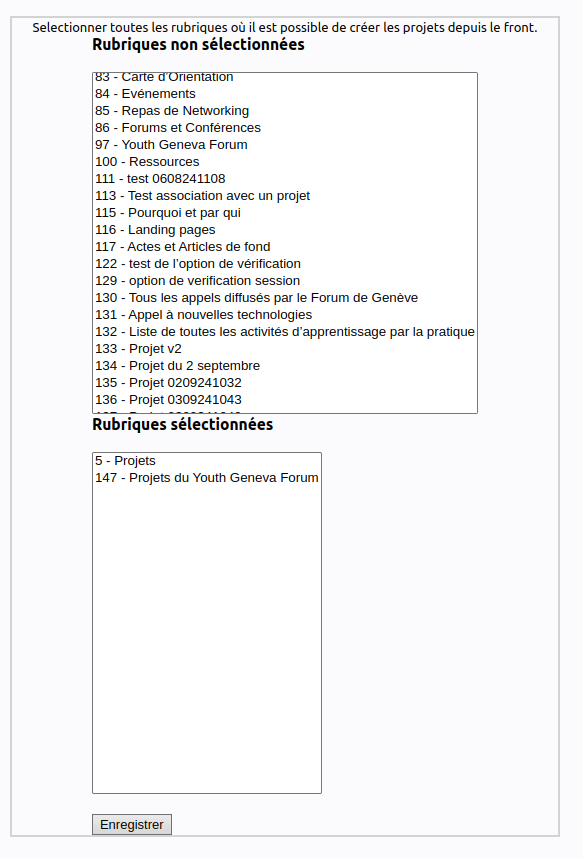
\includegraphics[trim=0 0 0 0, clip, width=0.4\textwidth]{./images/c1.png}
    \caption{Option 1 - Rubriques de création}
    \label{option1}
\end{figure}
\vspace{0.5cm}
% ///////////////////////////////////
\newpage

\textbf{Option 2 :} 
\begin{itemize}
    \item Configuration : \texttt{osip\_config\_demandes}
    \item Explication : Cette option limite la validation des demandes pour rejoindre un projet aux administrateurs du projet. Attention, il ne faut pas confondre un administrateur de projet et un administrateur SPIP.
\end{itemize}

\vspace{0.5cm}
\begin{figure}[h]
    \centering
    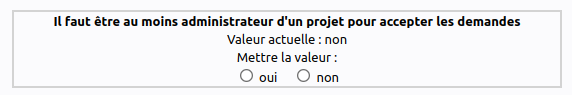
\includegraphics[trim=0 0 0 0, clip, width=1\textwidth]{./images/c2.png}
    \caption{Option 2 - Droits pour les demandes}
    \label{option2}
\end{figure}
\vspace{0.5cm}

% ///////////////////////////////////



\textbf{Option 3 :} 
\begin{itemize}
    \item Configuration : \texttt{osi\_projets/synchronisation\_mots}
    \item Explication : Dans le menu édition d'un projet, il existe la "\textit{Gestion des mots clés}" (Cf figure \ref{option3_bis}). Dans ce bloc, le premier bouton, intitulé "Mots-clés du projet", permet de synchroniser les mots-clés du projet à la rubrique associée (d'ajouter les mots clés du projet) et le deuxième l'inverse. Quand l'option 3 est activée, cette synchronisation prend en compte les groupes de mots-clés et ne rajoute que les mots-clés que l'autre groupe peut obtenir avec les règles des groupes de mots-clés.
\end{itemize}
\vspace{0.5cm}
\begin{figure}[h]
    \centering
    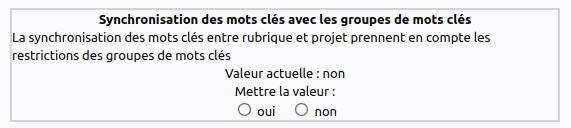
\includegraphics[trim=0 0 0 0, clip, width=1\textwidth]{./images/c3.png}
    \caption{Option 3 - Synchronisation avec les règles des groupes de mots}
    \label{option3}
\end{figure}
\vspace{0.5cm}
\begin{figure}[h]
    \centering
    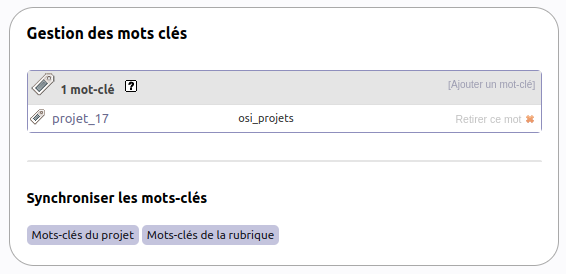
\includegraphics[trim=0 0 0 0, clip, width=0.7\textwidth]{./images/c3_bis.png}
    \caption{Menu de gestion des mots clés}
    \label{option3_bis}
\end{figure}

% ///////////////////////////////////
\newpage

\textbf{Option 4 :} 
\begin{itemize}
    \item Configuration : 
    \begin{itemize}
        \item \texttt{osi\_projets/types\_de\_mots/condition}
        \item \texttt{osi\_projets/types\_de\_mots/condition\_inverse}
        \item \texttt{osi\_projets/types\_de\_mots/recompense}
    \end{itemize}

    \item Explication : Dans le menu d'édition d'un projet, il est possible d'ajouter des mots clés à celui-ci. Dans la table \texttt{spip\_mots\_liens}, qui est la table qui permet de faire la liaison entre un mot et un objet (ici un projet), la colonne \texttt{lien\_projet} a été ajoutée. Cette colonne prend une valeur n qui permet de définir à quoi sert ce mot clé par rapport au projet.
    \begin{itemize}
        \item Conditions (n=2) : Les conditions sont des mots clés que l'auteur doit aussi avoir pour pouvoir rentrer dans le projet. Si l'auteur est déjà présent dans le projet mais qu'il ne respecte plus les conditions, rien n'est fait pour lui. Cependant, s'il y quitte le projet, il ne pourra plus revenir dedans tant qu'il ne respecte pas les nouvelles conditions. Ceci est possible grâce au filtre \texttt{filtre\_verifier\_conditions\_projet} utilisé dans le formulaire \texttt{ajouter\_auteur\_projet}, qui est le formulaire pour le front. Il faut donc faire attention, car le formulaire \texttt{ajouter\_autre\_auteur\_projet}, qui est celui utilisé dans le back office, permet lui en revanche d'ajouter un autre auteur dans le projet sans cette limitation.
        \item Conditions inverses (n=4) : Les conditions inverses fonctionnent avec le même principe que les conditions, sauf qu'ici il ne faut posséder aucune des conditions inverses pour rentrer dans un projet.
        \item Récompenses (n=3) : Les récompenses sont des mots clés que gagne un auteur quand, dans le menu édition du projet, on lui a donné les récompenses.
    \end{itemize}
\end{itemize}

\textbf{Remarque importante sur les récompenses :} Il faut faire attention avec les mots clés de "Récompenses". Dans l'état actuel du plugin, il est possible de "tricher" pour obtenir des mots clés de récompenses. En effet, un auteur peut ici créer un projet, ajouter autant de récompenses que de mots clés qu'il souhaite obtenir et se donner les récompenses (permission qu'il a car il est le créateur du projet). Dans l'état actuel du plugin, il est de la responsabilité du créateur du site de ne pas mettre en place un système de récompense s'il est possible de créer des projets sur le front par des personnes qui ne sont pas des personnes de confiance.


\vspace{0.5cm}
\begin{figure}[h]
    \centering
    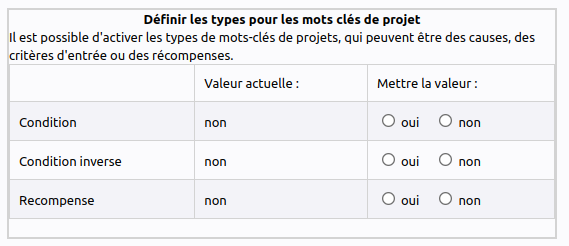
\includegraphics[trim=0 0 0 0, clip, width=1\textwidth]{./images/c4.png}
    \caption{Option 4 - Choix des types de mots clés}
    \label{option4}
\end{figure}
\vspace{0.5cm}


% ///////////////////////////////////


\textbf{Option 5 :} 
\begin{itemize}
    \item Configuration : \texttt{osi\_projets/verification\_projets}
    \item Explication : Cette option permet que tous les projets créés soient validés du côté back office pour les publier. Pour valider un projet, il faut se rendre dans la page d'édition des projets et modifier son statut.
\end{itemize}
\vspace{0.5cm}
\begin{figure}[h]
    \centering
    
\includegraphics[trim=0 0 0 0, clip, width=1\textwidth]{./images/c5.png}
    \caption{Cadre de l'option 5}
    \label{option5}
\end{figure}
\vspace{0.5cm}

\newpage
% ///////////////////////////////////


\textbf{Option 6 :} 
\begin{itemize}
    \item Configuration : \texttt{osi\_projets/recursivite}
    \item Explication : Lors de la création d'un projet, un mot clé est ajouté à ce projet qui correspond à l'id du projet (c'est un mot clé unique qui représente ce projet). Si cette option est activée, alors pour tout nouveau sous-projet, le mot clé représentant le projet père est ajouté en tant que condition au projet fils. Le bouton "\textit{Appliquer la récurrence sur tous les projets déjà existants}" permet de faire cela aussi pour les anciens projets. Si on a plusieurs projets à la chaîne, les projets doivent se faire dans l'ordre du projet le plus haut au sous-projet le plus profond.
\end{itemize}
\vspace{0.5cm}
\begin{figure}[h]
    \centering
    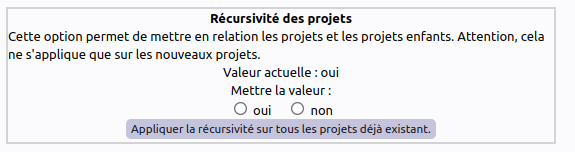
\includegraphics[trim=0 0 0 0, clip, width=1\textwidth]{./images/c6.png}
    \caption{Cadre de l'option 6}
    \label{option6}
\end{figure}
\vspace{0.5cm}

% ///////////////////////////////////

\textbf{Option 7 :} 
\begin{itemize}
    \item Configuration : \texttt{osi\_projets/webmaster\_droits}
    \item Explication : Cette option permet d'offrir les possibilités accordées aux administrateurs d'un projet aux administrateurs SPIP.
\end{itemize}
\vspace{0.5cm}
\begin{figure}[h]
    \centering
    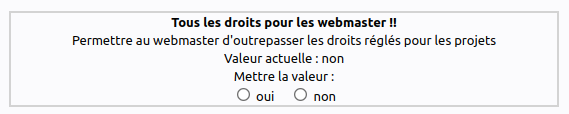
\includegraphics[trim=0 0 0 0, clip, width=1\textwidth]{./images/c7.png}
    \caption{Cadre de l'option 7}
    \label{option7}
\end{figure}

% ///////////////////////////////////
\newpage

\textbf{Option 8 :} 
\begin{itemize}
    \item Configuration : \texttt{osi\_projets/auteur\_banni}
    \item Explication : Cette option enlève tous les auteurs bannis de la liste des auteurs que l'on peut ajouter avec le formulaire \texttt{ajouter\_autre\_auteur\_projet}.
\end{itemize}
\vspace{0.5cm}
\begin{figure}[h]
    \centering
    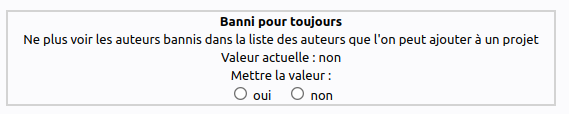
\includegraphics[trim=0 0 0 0, clip, width=1\textwidth]{./images/c8.png}
    \caption{Cadre de l'option 8}
    \label{option8}
\end{figure}

% ///////////////////////////////////

\textbf{Option 9 :} 
\begin{itemize}
    \item Configuration : \texttt{osi\_projets/creer\_sous\_projet\_int}
    \item Explication : Cette option permet aux administrateurs d'un projet de pouvoir créer un sous-projet sur le front. Cette utilisation est supplémentaire à celle de l'option 1.
\end{itemize}
\vspace{0.5cm}
\begin{figure}[h]
    \centering
    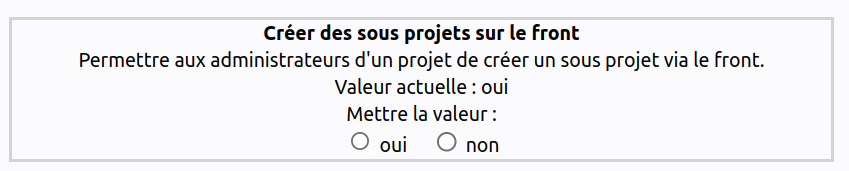
\includegraphics[trim=0 0 0 0, clip, width=1\textwidth]{./images/c9.png}
    \caption{Cadre de l'option 9}
    \label{option9}
\end{figure}


% ///////////////////////////////////
\newpage

\textbf{Option 10 :} 
\begin{itemize}
    \item Explication : Cette option est une sécurité qui permet de situer le projet sur le front quand aucune rubrique mère n'est définie lors de la création du projet. Si aucune rubrique n'est définie ici, le projet sera créé dans le sommaire.
\end{itemize}
\vspace{0.5cm}
\begin{figure}[h]
    \centering
    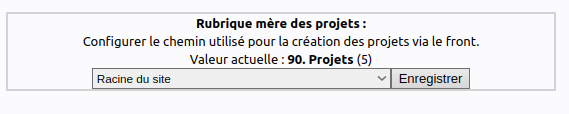
\includegraphics[trim=0 0 0 0, clip, width=1\textwidth]{./images/c10.png}
    \caption{Cadre de l'option 10}
    \label{option10}
\end{figure}

% ///////////////////////////////////
\newpage

\subsubsection*{Gestion des rôles} \label{subsubsection:gestion-roles}

Chaque membre d'un projet peut obtenir des rôles. Les rôles sont liés à un membre d'un projet. C'est-à-dire qu'un auteur peut avoir un rôle pour un projet et ne pas l'avoir pour un autre projet.\\
\newline
Le fichier \texttt{action/exemple\_roles} permet de voir la forme que peuvent avoir des rôles. Il est activable sur le back-office grâce au bouton "\textit{Utiliser les rôles d'exemple}". Les rôles d'exemple sont les suivants :


\vspace{0.5cm}

\begin{tabular}{|>{\centering\arraybackslash}m{6.2cm}|>{\centering\arraybackslash}m{6cm}|}
    \hline
    \rowcolor{lightgray} 
    Nom du rôle & Utilisation \\ 
    \hline
    \textbf{FORMATEUR} & Représente les personnes qui réalisent les formations \\ 
    \hline
    \textbf{SPONSOR} & Représente les personnes qui financent les projets \\ 
    \hline
    \textbf{EVALUATEUR PAR LES PAIRS} & Personne en lien avec le projet et qui sert à l'évaluer \\ 
    \hline
    \textbf{EVALUATEUR INDEPENDANT} & Personne pas directement en lien avec le projet et qui sert à l'évaluer \\ 
    \hline
\end{tabular}

\vspace{0.5cm}

Cependant, le but n'est pas forcément d'utiliser les rôles d'exemple, mais plutôt de créer des rôles adaptées à l'utilisation du plugin.\\
\newline
Un rôle possède trois caractéristiques.
\begin{itemize}
    \item Le titre du rôle (obligatoire) : cela permet de l'identifier, on ne peut pas avoir deux rôles avec le même titre.
    \item La description du rôle : permet d'expliquer le but du rôle.
    \item La question : c'est la question qui est posée dans le formulaire de demande pour rejoindre le projet (\textit{ajouter\_auteur\_projet}) pour rejoindre avec ce rôle. 
\end{itemize}
Une fois qu'un rôle est créé, il faut penser à cliquer sur le bouton "\textit{Rendre le rôle actif}" pour pouvoir utiliser le rôle. Initialement, le rôle est inactif.

\subsubsection*{Gestion des notifications} \label{subsubsection:gestion-notifications}

Pour pouvoir utiliser la partie notification du plugin, il faut installer le plugin \href{https://plugins.spip.net/notifavancees.html}{Notifications avancées}.\\
\newline
Il existe deux types de notifications : les notifications individuelles et les notifications de groupe. Les notifications individuelles s'adressent à la personne qui est concernée, généralement la personne qui essaie de rejoindre un projet. Les notifications de groupe s'adressent ici à l'ensemble des personnes du projet.\\
\newline
Les notifications se trouvent toutes dans la rubrique \textit{notifications}.

\subsection{Menu édition} \label{subsection:menu-edition}

Dans le menu d'édition, on retrouve les différentes possibilités de gestion et de modification d'un projet précis.

\begin{itemize}
    \item La gestion des mots clés : permet de rajouter un mot clé et de modifier son type (Cf. option 4).
    \item La gestion des demandes : on trouve ici les demandes pour rejoindre le projet et les demandes pour obtenir un rôle. Seuls les membres ayant au minimum des droits administrateurs peuvent accepter (ou refuser) les demandes. 
    \item La gestion des membres du projet : permet de modifier le rôle ou les droits d'un membre d'un projet. C'est aussi ici qu'on peut exclure un membre du projet.
\end{itemize}
